%%%%%%%%%%%%%%%%%%%%%
% Short Sectioned Assignment
% LaTeX Template
% Version 1.0 (5/5/12)
%
% This template has been downloaded from:
% http://www.LaTeXTemplates.com
%
% Original author:
% Frits Wenneker (http://www.howtotex.com)
%
% License:
% CC BY-NC-SA 3.0 (http://creativecommons.org/licenses/by-nc-sa/3.0/)
%
%%%%%%%%%%%%%%%%%%%%%

%----------------------------------------------------------------------------------------
%	PACKAGES AND OTHER DOCUMENT CONFIGURATIONS
%----------------------------------------------------------------------------------------

\documentclass[paper=a4, fontsize=11pt]{scrartcl} % A4 paper and 11pt font size

\usepackage{graphicx}
\usepackage[T1]{fontenc} % Use 8-bit encoding that has 256 glyphs
\usepackage{fourier} % Use the Adobe Utopia font for the document - comment this line to return to the LaTeX default
\usepackage[english]{babel} % English language/hyphenation
\usepackage{amsmath,amsfonts,amsthm} % Math packages

\usepackage{lipsum} % Used for inserting dummy 'Lorem ipsum' text into the template

\usepackage{sectsty} % Allows customizing section commands
\allsectionsfont{\centering \normalfont\scshape} % Make all sections centered, the default font and small caps

\usepackage{fancyhdr} % Custom headers and footers
\pagestyle{fancyplain} % Makes all pages in the document conform to the custom headers and footers
\fancyhead{} % No page header - if you want one, create it in the same way as the footers below
\fancyfoot[L]{} % Empty left footer
\fancyfoot[C]{} % Empty center footer
\fancyfoot[R]{\thepage} % Page numbering for right footer
\renewcommand{\headrulewidth}{0pt} % Remove header underlines
\renewcommand{\footrulewidth}{0pt} % Remove footer underlines
\setlength{\headheight}{13.6pt} % Customize the height of the header

\numberwithin{equation}{section} % Number equations within sections (i.e. 1.1, 1.2, 2.1, 2.2 instead of 1, 2, 3, 4)
\numberwithin{figure}{section} % Number figures within sections (i.e. 1.1, 1.2, 2.1, 2.2 instead of 1, 2, 3, 4)
\numberwithin{table}{section} % Number tables within sections (i.e. 1.1, 1.2, 2.1, 2.2 instead of 1, 2, 3, 4)

\setlength\parindent{0pt} % Removes all indentation from paragraphs - comment this line for an assignment with lots of text

%----------------------------------------------------------------------------------------
%	TITLE SECTION
%----------------------------------------------------------------------------------------

\newcommand{\horrule}[1]{\rule{\linewidth}{#1}} % Create horizontal rule command with 1 argument of height

\title{	
\normalfont \normalsize 
\textsc{CS 472 Evolutionary Computation} \\ [25pt] % Your university, school and/or department name(s)
\horrule{0.5pt} \\[0.4cm] % Thin top horizontal rule
\huge Project 2 \\ % The assignment title
\horrule{2pt} \\[0.5cm] % Thick bottom horizontal rule
}

\author{Alex Cochrane} % Your name

\date{\normalsize\today} % Today's date or a custom date

\begin{document}

\maketitle % Print the title

%------------------------------------------------

%\horrule{0.5pt} \\[0.4cm] % Thin top horizontal rule
\section{Abstract}

%------------------------------------------------

\paragraph{} For this project we were tasked with adding functionality to create a Genetic Program that had certain functionality and could easily be expanded upon later. Doing this in C++ I chose to do the typing of individual nodes through polymorphism and inheritance. I decided it would be easiest to build my individuals up as abstract nodes. The nodes themselves will be typed off of there operation. Therefore when I build my populations of individuals I really just have to build a population of nodes and I will not have to worry about their types.

%------------------------------------------------

\horrule{0.5pt} \\[0.4cm] % Thin top horizontal rule
\section{Algorithm and Individual Description}

%------------------------------------------------
\paragraph{} For now there are only operations for building up a population of individuals, getting there fitness and removing/copying them. The easiest way to show how these methods work is to show the class diagram for there creation and then do pseudo code for the functions that need an explanation. This class diagram shows both how individuals, or nodes in my code, are formed and structured as well as the population of individuals. For now since all we need is to print out average size and average fitness as well as our best fitness, I have just created these functionalities in my population.

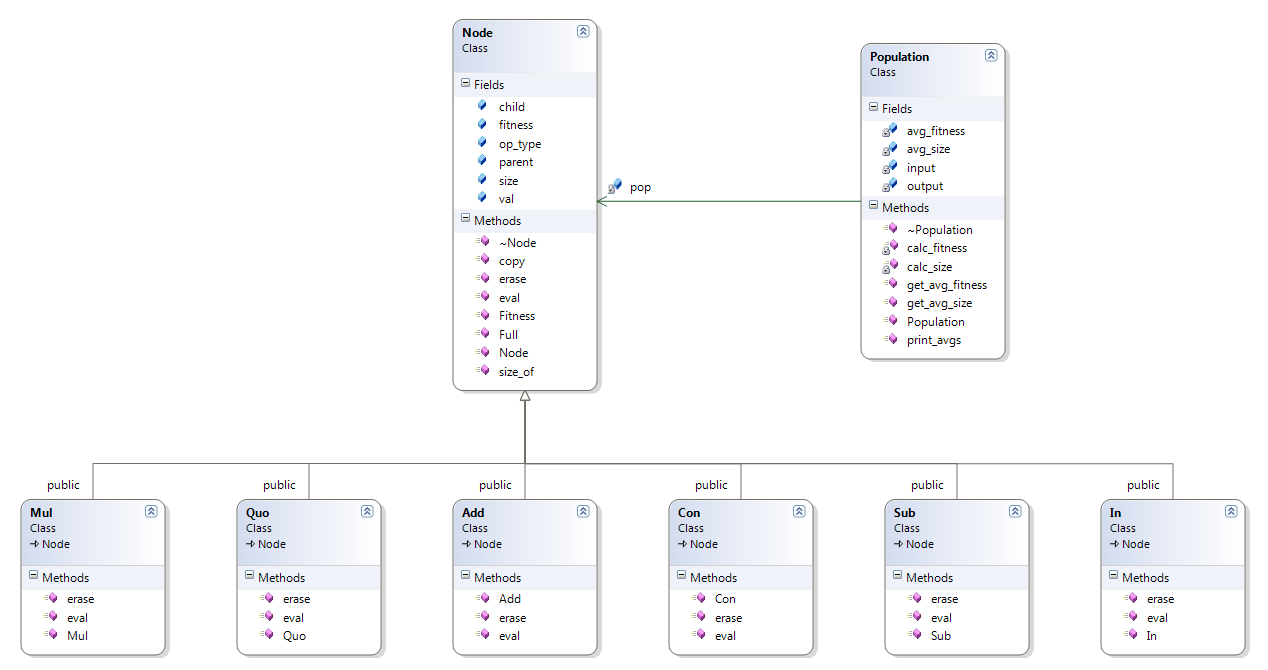
\includegraphics[scale=.5]{ClassDiagram}

\paragraph{} As the diagram shows, each node has the capability of being an addition, subtraction, multiplication, division, constant, and an input. The general attributes of a Node are its fitness, size, children, parent, and for certain individuals average fitness, average size, and value are necessary. These attributes are set by functions and will be discussed more during the following algorithm descriptions.

\paragraph{Pseudo Code: Copy}
\begin{verbatim}
temp = new Node(); // based off of t's op type
temp->attr = t->attr; // save over details about t so we have an exact copy
while all children have not be reached
    temp->child = temp->copy( t->child );
return temp;
\end{verbatim}

\paragraph{} This function is the only reason why I have to keep track of types in my solutions. Without this I would not have to worry about them at all. But nonetheless we have to create a new node and therefore we have to return a node at the end. therefore we cannot just have a straight copy, we have to return it from the function. This is one of the negatives to my solution. What it actually does is create the new node based on the type of the source. It then copies over all the details from the source into the new one including type, value, and children.

\paragraph{Pseudo Code: Evaluate}
\begin{verbatim}
// if non term
return eval(child[0]) op eval(child[1]); // where op is the operator based off of which node we are in
// if const
return val; // Our constant value
// if input
return in; // return the input value for evaluation
\end{verbatim}

\paragraph{} For evaluation of non terminals we want to return the evaluation of the right and left branches of the tree using the op for what node it is to perform an operation on the two returned values. If it is a constant we return a constant value generated on creation of the tree and if we are input we return the value of the input given on the call to evaluation.

\paragraph{Pseudo Code: Erase}
\begin{verbatim}
// if non term
while all children are deleted
    child->erase();
delete this;
return;
// if const or input
delete this; // we don't have children
return;
\end{verbatim}

\paragraph{} If we are a non terminal we need to erase our children. If we are a constant or an input we can just delete ourselves and return because we have no children.

\paragraph{Pseudo Code: Size}
\begin{verbatim}
temp = 1; // size
while all children have not been looked at
    if( child != NULL )
        temp += size( child );
    else // child == NULL const or input
        temp = 1;
size = temp; // local assignment so it is saved in the node/individual
return temp; // this returns so we can calculate
\end{verbatim}

\paragraph{} The essence of this code is that it uses recursion to go down to the end nodes and build up the size from the bottom. If the node is a constant or input node, we can say it is of size one and start returning up our recursive calls that were made when we were non terminals.

\paragraph{Pseudo Code: Full}
\begin{verbatim}
parent = node // this is the node passed in

if depth is not greater then our max depth
    while all children are not filled
        generate a random individual // Add,Sub,...
        call full( depth+1, this); // Fill the child
else at max depth
    while all children are not filled
        generate a random individual // Constant or input
\end{verbatim}

\paragraph{} This can be used to fill an entire individual structure. If we are not yet at max depth we add nodes that are ops, otherwise we add values that are either constants or input values. This is a quick and effective way at generating the tree, especially when we need to generate multiple ones.

\paragraph{} Now I will go into the functions that will be used by the population to compute fitness and size values. This list of functions will be expanded to include our future mutation and crossover functions. For now however we just have the ability to get at fitnesses and sizes, which automatically calculate the fitness and size values when trying to retrieve them. Another function prints out these values in a nice way.

\paragraph{Pseudo Code: Population}
\begin{verbatim}
// for when a new population is created
while pop is not full
    generate a new random node;
    node->full();
// set inputs and outputs
while inputs not full
    input[i] = i+1;
    output[i] = (i+1) * (i+1);
// get the avg_size and avg_fitness as well as best fitness of the pop
calc_size;
calc_fitness;
\end{verbatim}

\paragraph{} This generates the entire population with random individuals using the functions discussed earlier for creating a full tree. Then it sets up the input and output vectors used in creating fitness. Then it calculates the size of the trees as well as the fitness giving averages for both and a best fitness. The calculations are shown just below.

\paragraph{Pseudo Code: Get / Calculate Size / Fitness}
\begin{verbatim}
calc_size / calc_fitness
return avg_size / avg_fitness
// calc_size
avg_size = 0;
for( k = 0; k < population_size; k++)
    avg_size += pop[k]->size_of(pop[k]);
avg_size / population_size;
// calc_fitness
avg_fitness = 0;
for( k = 0; k < population_size; k++)
    temp = pop[k]->size_of(pop[k]);
    if( temp < best_fitness)
        best_fitness = temp;
        best_index = k;
    avg_fitness += temp;
avg_fitness / population_size;
\end{verbatim}

\paragraph{} So every time you try and access these values they are calculated that way we don't need to worry about wrong values being returned. This might be slower but it is more accurate and mistakes will be made less often this way. The calculation of size simply gets the size of each of the individuals and divides by the population size. For fitness however, it also stores the best fitness and its index, this will be important later for elitism.

\paragraph{Pseudo Code: Print}
\begin{verbatim}
calc_size();
calc_fitness();

cout << "These are the average values:" << endl;
cout << "Average Size: " << avg_size << endl;
cout << "Average Fitness: " << avg_fitness << endl;
cout << "Best Fitness: " << best_fitness << endl;
\end{verbatim}

\paragraph{} This is simply for testing purposes and is nice to have as a procedure instead of having to do it continually by hand.

%------------------------------------------------
\pagebreak
\horrule{0.5pt} \\[0.4cm] % Thin top horizontal rule
\section{Results}

%------------------------------------------------

\paragraph{} The following results show that everything is working as well as it should right now. The average fitness is extremely high right now because when a divide by zero happens I return 9 million in hopes of making that fitness really large. This is not ideal and when we actually do some more work with this I will adjust my penalty accordingly. The average size is always the same because for now all the trees are identical full trees, the nodes themselves are the only differences. When we perform crossover or mutation hopefully we will start to get a varying size to the trees.

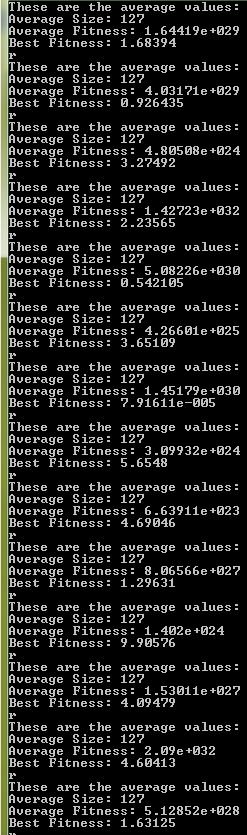
\includegraphics{Results}

%------------------------------------------------

\horrule{0.5pt} \\[0.4cm] % Thin top horizontal rule
\section{Conclusion}

%------------------------------------------------

\paragraph{} For now my set up is working as expected. I will try to start adding selection, crossover, and mutation to test it further but for now it seems to be functioning perfectly. Without the real tests to the system like crossover or mutation there really isn't much more to do for this project.

%------------------------------------------------

\horrule{0.5pt} \\[0.4cm] % Thin top horizontal rule
\end{document}
